\documentclass{article}

\usepackage{arxiv}
\usepackage[utf8]{inputenc} % allow utf-8 input
\usepackage[T1]{fontenc}    % use 8-bit T1 fonts
\usepackage{hyperref}       % hyperlinks
\usepackage{url}            % simple URL typesetting
\usepackage{booktabs}       % professional-quality tables
\usepackage{amsfonts}       % blackboard math symbols
\usepackage{nicefrac}       % compact symbols for 1/2, etc.
\usepackage{microtype}      % microtypography
\usepackage{cleveref}       % smart cross-referencing
\usepackage{lipsum}         % Can be removed after putting your text content
\usepackage{graphicx}
\usepackage{natbib}
\usepackage{doi}
\usepackage{listings}
\usepackage{caption}
\usepackage{subcaption}

\title{Colonies - Compute Continuums across Platforms}

\author{{\hspace{1mm}Johan Kristiansson} \\
	Department of Computer Science \\
	RISE Research Institutes of Sweden \\
	Luleå, Sweden \\
	\texttt{johan.kristiansson@ri.se} \\
	\And
	{\hspace{1mm}Thomas Ohlson Timoudas} \\
	Department of Computer Science \\
	RISE Research Institutes of Sweden \\
	Luleå, Sweden \\
	\texttt{thomas.ohlson.timoudas@ri.se} \\
	\And
	{\hspace{1mm}Henrik Forsgren} \\
	Department of Computer Science \\
	RISE Research Institutes of Sweden \\
	Luleå, Sweden \\
	\texttt{thomas.ohlson.timoudas@ri.se} \\
	\And
	{\hspace{1mm}Erik Källman} \\
	Department of Computer Science \\
	RISE Research Institutes of Sweden \\
	Luleå, Sweden \\
	\texttt{erik.kallman@ri.se} \\
}

% Uncomment to override  the `A preprint' in the header
\renewcommand{\headeright}{Technical Report}
\renewcommand{\undertitle}{Technical Report}
%\renewcommand{\shorttitle}{\textit{arXiv} Template}

%%% Add PDF metadata to help others organize their library
%%% Once the PDF is generated, you can check the metadata with
%%% $ pdfinfo template.pdf
\hypersetup{
pdftitle={A template for the arxiv style},
pdfsubject={q-bio.NC, q-bio.QM},
pdfauthor={David S.~Hippocampus, Elias D.~Striatum},
pdfkeywords={First keyword, Second keyword, More},
}

\begin{document}
\maketitle

\begin{abstract}
Artificial intelligence and machine learning has gained significant traction in recent years. At the same time, development and operation of AI workloads has become increasingly challenging. One difficulty is the lack of portability, making it cumbersome to move from one platform to another. Creating and operating fully automated end-to-end workflows across devices, edge, and cloud platforms is even more challenging.

To address the aforementioned challenges, the paper introduces a framework termed Colonies which is available as open-source\footnote{https://github.com/colonyos/colonies} and designed to facilitate execution of computational workloads across a diverse range of platforms. It can be used to implement grid-alike distributed virtual computer systems, and is founded upon a loosely-coupled microservice architecture that beaks down complex workflows into composable functions. With the use of an HTTP protocol, these composable functions can be implemented in any computer language and be executed by independent executors deployed across various systems, e.g. cloud, edge, devices, or even in web browsers. Colonies orchestrates the execution and by using a zereo-trust security protocol, a collection of distributed executors can function as a single cohesive unit, thereby establishing seamless compute continuums across multiple platforms.

In addition to a technical description of the Colonies framework, the paper also describes some potential use cases. The paper describe how Colonies can be leveraged to build a remote sensing platform on Kubernetes, serve as a building block for edge computing, implement a serverless FaaS (Function-as-a-Service), and how it can be integrated with HPC platforms. Finally, the paper presents a performance investigation, as well as scalability and robustness evaluation. 

In summary, Colonies is a highly versatile and scalable framework that can streamline development and deployment of computational workloads across heterogeneous platforms while ensuring full traceability and zero-trust security.
\end{abstract}

% keywords can be removed
\keywords{Serverless computing \and Parallel computing \and Workflow orchestration}

\section{Introduction}
Developing robust and scalable AI systems is a challenging task that requires deep understanding in several fields. To begin with, an AI model must be trained which requires knowledge in advanced statistics or machine learning, as well as access to training and validation data. Typically, this data must be pre-processed through various stages before it can be utilized. Although it may be practical for small-scale projects to run the entire training processes on local development computers, larger AI models typically require access to powerful compute clusters or even HPC systems. Manual use of such infrastructure can be laborious and time-consuming. Automating the training process enables faster iterations and quicker discovery of useful models.

Taking an AI model into production requires substantial software engineering expertise. In contrast to traditional IT workloads, both the data and the model must be managed in addition to the software itself. As most models require regular re-training or re-calibration, it must be possible to update deployed models and software seamlessly without losing information or breaking the system. In many cases, there is a constant flow of data ingested into the system which must be managed even in case of failures. This becomes even more challenging when nodes or parts of the underlying infrastructure become unavailable due to maintenance such as software updates, hardware replacements and sometimes missconfiguration problems.

In some cases, it may be necessary to scale the system to increase or reduce the capacity. This is especially critical when using expensive cloud resources. Scaling the system means that the underlying infrastructure may change at any time, causing instability issues for running services or workflows. Therefore, it must be possible to detect failed computations and reprocess failed tasks part of a larger workflow. Workflows must hence be designed to handle an ever-changing infrastructure, and if a failed computation cannot be restored gracefully, engineers must be able to quickly perform root cause analysis to manually recover the system.

In reality, AI system requires integration of multiple systems. For instance, data need to be captured from an IoT system or pulled from third-party database running on different domains than the compute cluster. With the emergence of edge computing, parts of a data pipeline may also run on edge servers to bring computations closer to data sources. Configuring and setting up such pipelines add even more complexity.

Additionally, many compute clusters operate on-premises installations. Sometimes it is necessary to temporarily increase the capacity of on-prem clusters by combining resources from multiple providers, for example, adding cloud compute resources to handle peak loads or utilize HPC resources to quickly reprocess historical data. Developing hybrid workflows where some jobs run in the cloud and others run on HPC systems requires even more software development efforts and is beyond the scope of most users, preventing them from utilizing powerful hardware. Clearly, there is a need for a framework that can consolidate various platforms to simplify development and enable seamless execution across platforms.

This paper presents a framework called Colonies, specifically designed for implementing distributed virtual computer systems that facilitate integration with other systems. Colonies is built around a loosely-coupled microservices architecture that separates workflow definitions from implementation and deployment, offering a modern approach to grid computing. The main objective is to create a tool where monolithic workflows can be broken down into independent and separated compute units that can be dynamically added or removed while executing workflows. These compute units can be implemented in any computer language and easily integrated with other systems, and then be deployed anywhere on the Internet. The remainder of the paper describes the Colonies framework and how it can be used to create robust and scalable AI systems. 

\section{Related work}
Workflow management has been extensively studied in both academic and industrial settings with numerous approaches proposed to address the challenges in this field. For example, Apache Airflow \cite{apache_airflow} is a popular open-source workflow management system for handling data engineering pipelines. Like Colonies, Apache Airflow enables developers to create custom operators and executors that can be integrated with various systems. Additionally, Apache Airflow offers an HTTP API that makes it possible to develop software development kits (SDKs) in various programming languages. However, Apache Airflow does not realy on a queuing system. Instead, it must be integrated with a message broker, such as RabbitMQ \cite{rabbitmq} or Kafka \cite{apache_kafka}, to implement task queues, resulting in a more complex architecture than Colonies. Furthermore, Colonies is based on a distributed microservice architecture that makes it more suitable for DevOps software development. As Colonies is loosely coupled, executors can be implemented and dynamically deployed without reconfiguring the workflow engine, effectively turning it to a grid computing platform. 

Argo \cite{argowf} is an open source container-native workflow engine for orchestrating parallel jobs on Kubernetes. It is can be used for running CI/CD pipelines or compute intensive machine learning or data processing tasks where each job runs as a container. In contrast, Colonies offers a more versatile approach, allowing jobs to be launched within a container. As launching new containers on Kubernetes can occasionally be time-consuming, Colonies can delivers higher throughput as the costs of starting new jobs are minimal. This is particular useful when launching large container images, or workloads (e.g. Julia scripts) or that takes relative long time to start. 

OpenWolf \cite{openwolf} is a serverless workflow engine designed to utilize the Function-as-a-Service (FaaS) paradigm for composing complex scientific workflows. It is based on OpenFaaS \cite{openfaas}, which allows functions to run on Kubernetes clusters. In contrast, Colonies does not require Kubernetes, but provides a zero-trust security protocol to allow functions to be executed securely by distributed executor workers deployed anywhere on the Internet.

The serverless workflow project \cite{serverlessworkflows} aims at providing a vendor-neutral workflow DSL. Synapse \cite{synapse} is a workflow management system similar to Argo, but that implements the serverless workflow specification. A similar engine is proposed in \cite{scafe}. It is important to point out that Colonies does not provide an infrastructure for function execution. Instead, Colonies primary role is to serve as a platform for coordinating function executions, which are carried out by distributed executor.

J. Represa et al. \cite{GarciaRepresa1740746} explore various challenges associated with developing microservice-based workflow management for industrial automation within the context of the Arrowhead project. The authors conclude that microservice-based workflow technologies is viable for industrial applications, particularly due to their inherent flexibility. The primary contribution of this paper is a comprehensive technical description of how to implement a distributed workflow engine based on microservice principles, extending beyond orchestrating microservices to execute automation tasks.

Grid computing is a distributed computing model that allows multiple computers, sometimes geographically distributed, to work together as a cohesive system to solve large-scale computational problems. It can be used to harness resources from numerous computers to solve complex tasks.


\section{The Colonies framework}
\label{sec:headings}
Microservices is an architectural design pattern in which an application is structured as a collection of small, independently deployable, and loosely coupled services that communicate with other microservices through a well-defined API. By dividing the application into smaller, focused microservices, applications become easier to understand, maintain, and develop. Each microservice can be scaled independently, making it easier to handle increased demand for a certain service. Additionally, different microservices can be developed by using diverse technologies, frameworks, or programming languages, enabling developers to select the most suitable tools for each specific problem. By assigning ownership of specific microservices to individual teams, it also becomes easier to coordinate work and maintain a consistent development process.

Currently, microservices are primarily used to implement large-scale web applications or Internet applications requiring high-availability. It has not yet become a prevalent design principle for workload management or implementation of HPC applications. Instead, simple job scripts are commonly used. In some cases, message brokers (e.g., RabbitMQ) are used to build worker queues to distribute tasks among multiple workers. Although this approach may be effective for simpler applications, creating dependencies between tasks, such as controlling the order of execution or passing information between tasks is not straightforward.

Colonies is based on a microservice architecture where workflows are decomposed into a set of independent functions. An example of a function could for example be a function that trains a neural network, prepare a batch of data, or upload inferred results to a third-party database etc. An executor is responsible for executing one or several functions, making it very simular to a microservice. All coordination is managed by a cluster of Colonies servers, allowing complex workflows to be broken down into independent functions that can be developed and tested separately. Analogous to traditional microservices, scalability can be achieved simply by adding more executors implementing the same function specification. If an executor crashes during task execution, the task is automatically reassigned to another executor. 

\subsection{The role of queues as seperation of concerns}
Separation of concerns (SoC) is a fundamental design principle in computer science that aims to break down a complex software system into smaller, more manageable parts. For example, HTTP APIs can be used to abstract away implementation detail and provide a clear and simple interface for interacting with a particular service. However, HTTP protocols alone are insufficient for handling dynamic environments where components frequently fails or the underlying infrastructures is constantly changing. To address such environments, an alternative mechanism is necessary. 

Queues enable software services to communicate indirectly by acting as a buffer between them. Queues makes it possible to decouple each executor and make them operate independently, e.g. an executor can be updated or replaced without affecting other executors. Queues also allow for asynchronous communication between executors, enabling them to process tasks at their own pace. This ensures that slower executors do not bottleneck faster ones, leading to a more efficient and scalable system. Most importantely, queues enable load balancing by distributing tasks among multiple executors, thus making it possible to parallelize workflow execution. 

Queues can be implemented in different ways, and while message brokers are a common solution, Colonies adopts an alternative strategy and leverage a standard database and querying it for tasks to assign to different executors. One key advantage of this approach is that it enables fine-grained task assignments, making it possible to assign specific tasks to particular executors. For instance, an executor of the browser type can be limited to only executing tasks of the browser type. This level of granularity cannot easily be implemented using message brokers which generally do not offer introspection of queue, or provide the ability to pull specific messages out of the queue. Generarally, the only way to retrieve a specific message is to pull all messages from the queue, obtain the message, and then place all remaining messages back into the queue in the same order. In contrast, a database can also function as a queue and a query can match any columns thus making it possible to assign specific executors to processes.

\begin{equation}
    \label{eq:pt}
    priority_{time}=submission_{time} - priority \cdot 10^9 \cdot 60 \cdot 60 \cdot 24
\end{equation}

Implementing queue functionality using a database can be achieved in SQL by utilizing the \emph{order by timestamp} and \emph{limit 1} clauses to select tasks according to their submission times. Upon submission of a task, a \emph{priority time} value is computed and stored in the database. The primary objective of the priority time is to modify the submission timestamp by subtracting a delta time calculated as a function a priority value. This enables prioritization of more critical tasks. Equation \ref{eq:pt} shows how the priority time is calculated for a nanosecond timestamp. 

\begin{figure}
     \centering
     \begin{subfigure}[b]{0.3\textwidth}
         \centering
         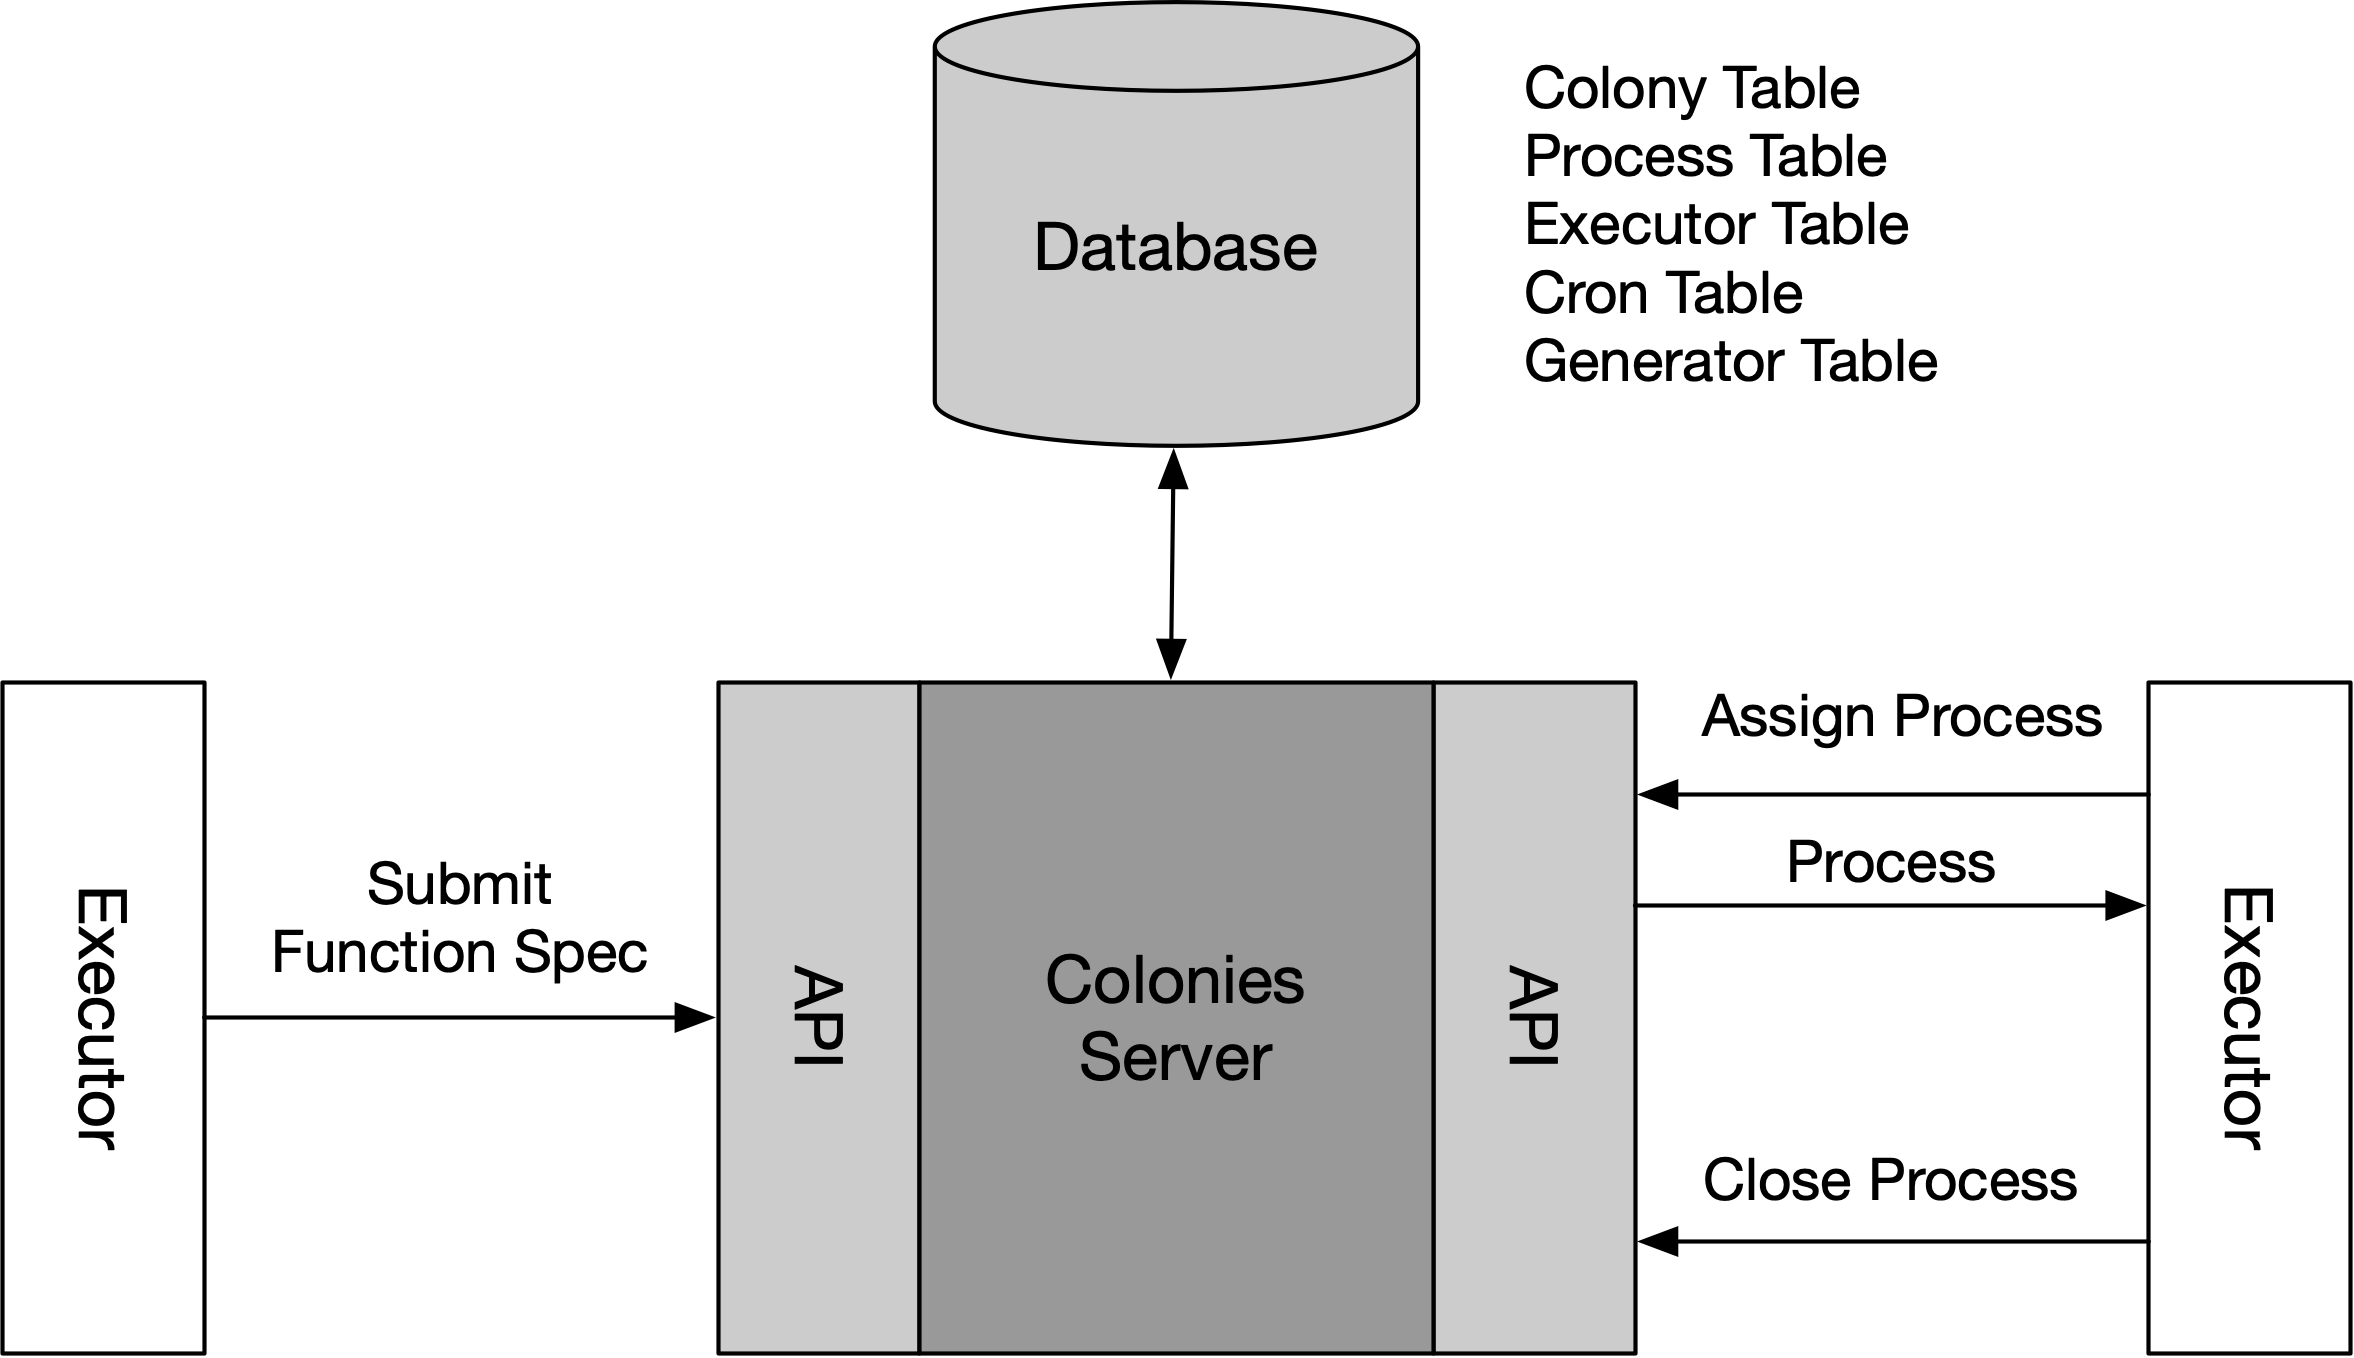
\includegraphics[scale=0.37]{arch.png}
         \caption{Process assignment steps.}
     \end{subfigure}
     \hfill
     \begin{subfigure}[b]{0.3\textwidth}
         \centering
         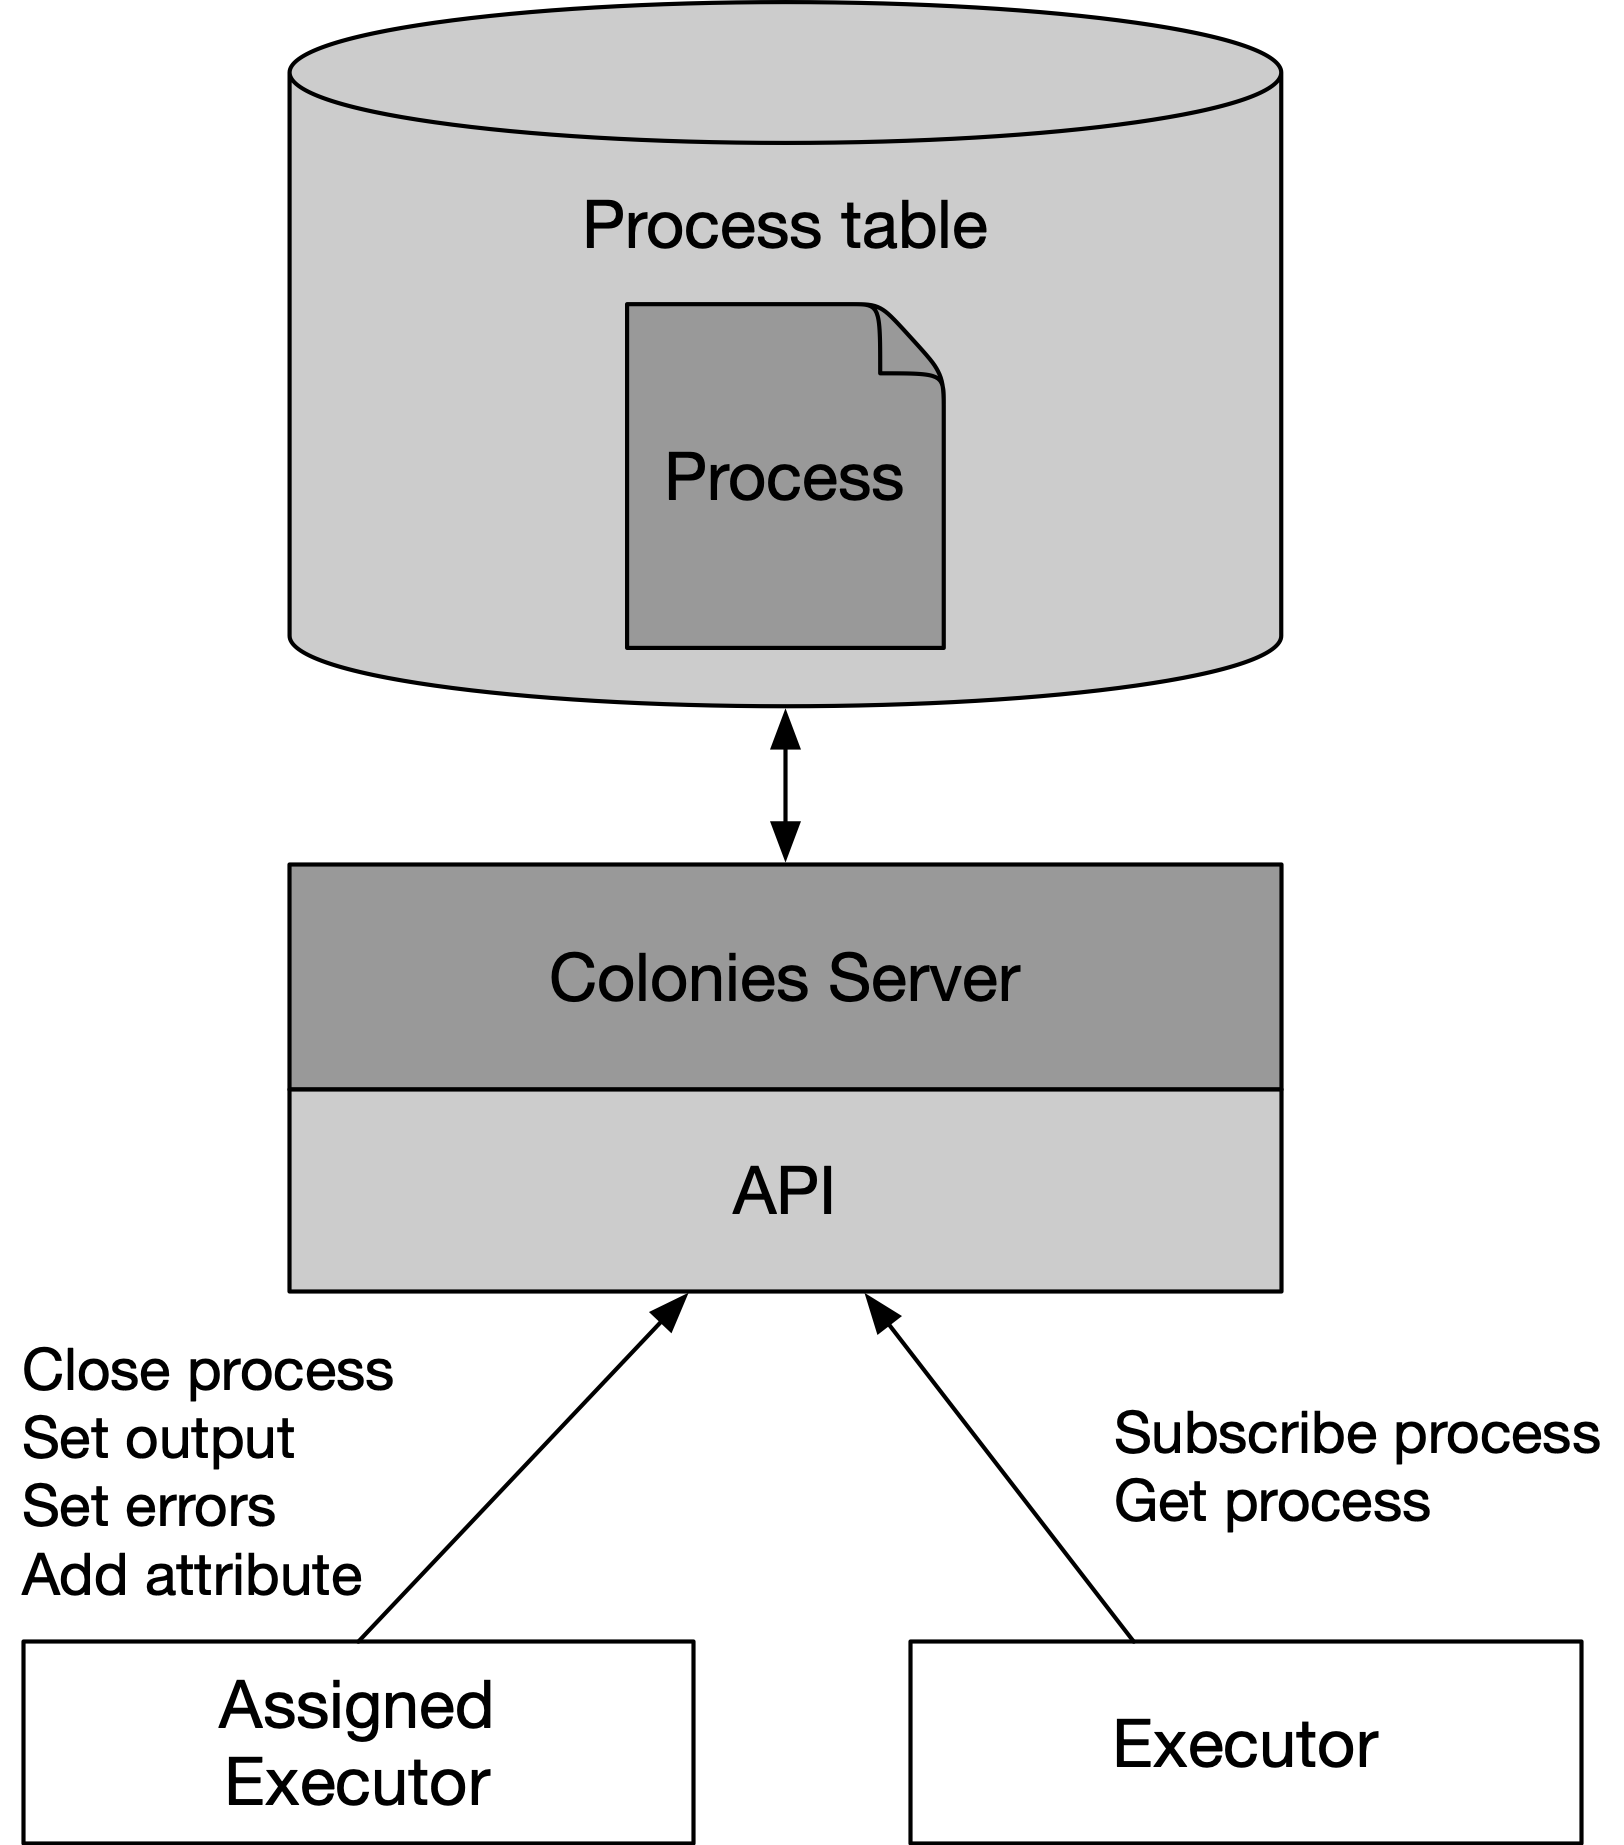
\includegraphics[scale=0.37]{process.png}
         \caption{Manipulation of a process.}
     \end{subfigure}
     \caption{Process management via Colonies HTTP API. Note that only the assigned executor has write access to the process database entry.}
     \label{fig:process_assignment}
\end{figure}

\subsection{Process tables}
Colonies provides a platform for executors to interact with each other by enabling them to submit function specifications to a Colonies server. Once submitted, other executors can connect to the server to receive execution assignments. When a function specification is submitted to the Colonies server, it is store as a process entry in a process table database. In this case, a process is similar to a task or a job, but also contains contextual information about the execution, for example, execution status (waiting, running, successful, failed), assigned executor ID, submission time, execution time, deadlines, priority etc. It also contains input and argument values as well as return values from the function innovation. In the remainder of the paper, we are going to use the term process instead of task or job.

The Colonies server acts as a job broker for executors, almost like an employment agency for people. When an executor connects to the Colonies server, the server hang the incomming HTTP connection\footnote{An alternative protocol is to use WebSockets or gPRC to communicate with the Colonies server.} until the executor is assigned a process, or until a connection timer expires. Note that the Colonies server does not connect to any executor. Rather, it is the responsibility of the executors to connect to the Colonies server. This enables executors to be deployed anywhere on the Internet, behind firewalls, commercial telco networks, or even in web browser-based applications.

Figure \ref{fig:process_assignment} illustrates an executor submitting a function specification that is later assigned to another executor. When registering, executors have to specify to the Colonies server which functions they are capable of executing. The Colonies server makes sure that the conditions (i.e requirmenets) of a function specification matches the capability of an executor. Note that the executors are responsibility of interpreting the assigned process and function specification to execute relevant code.

\begin{figure}[h]
	\centering
    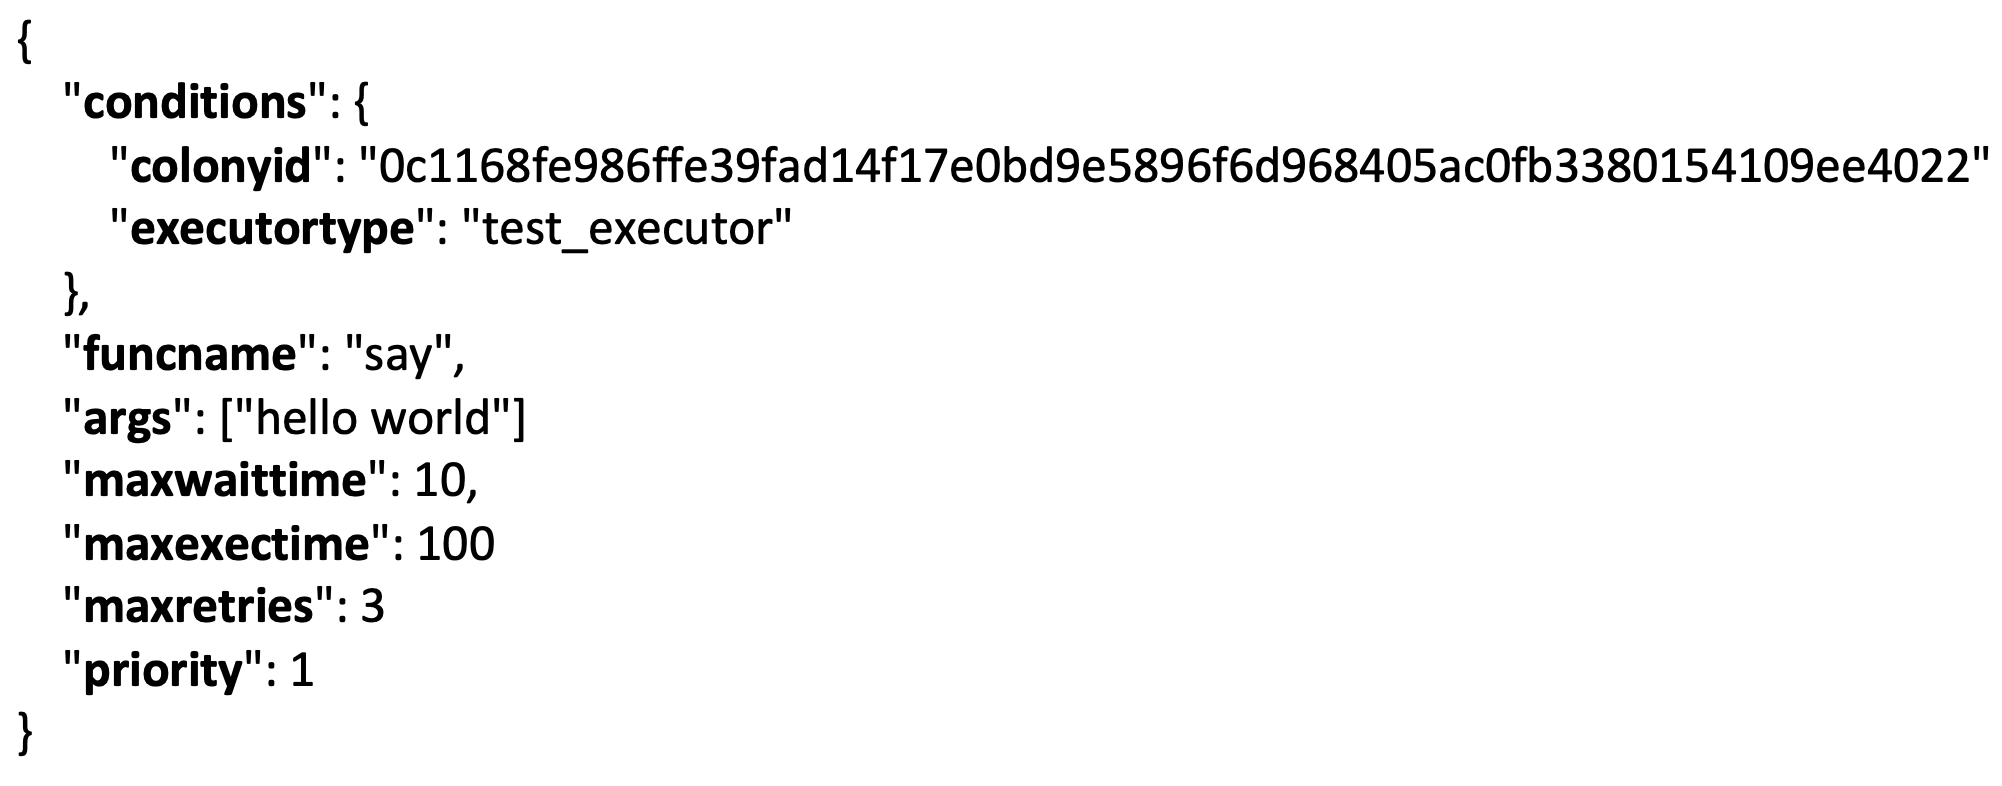
\includegraphics[scale=0.35]{function_spec.png}
	\caption{Example of a function spec.}
	\label{fig:function_spec}
\end{figure}

\subsection{A stateless failsafe mechanism}
The primary objective of all Colonies API requests is to alter a state stored in the database or retrieve information from the database. The Colonies framework is designed to be stateless, meaning that the Colonies server does not keep any information between requests. In other words, each request is handled independently, without relying on any information from previous requests. 

Figure \ref{fig:function_spec} shows an example of a function specification. The \emph{maxexectime} attribute specifies the maximum time an executor may run a process (in this case, 100 seconds). Before a process is assigned to an executor, the Colonies server updates the process entry in the process table database and calculates a deadline for when the process must be finished. The server then regularly checks for any running processes that have exceeded their deadlines. If such process is detected, it is reset, allowing it to be re-assigned to other executors. 

Making it possible to specify maximum execution time is a simple but powerful mechanism. To scale up a system, more executors can simply be deployed. Scaling down, however, can be more challenging. One solution is to select a set of executors to be removed and then starv them out by denying them new process assignments. Another, simpler solution, is to immediately destroy the executors and use the \emph{maxexectime} failsafe mechanism move back failed processes to the queue.  

The \emph{maxexectime} failsafe mechanism ensures that processes will eventually be executed even in the case of failures. This mechanism also relieves the burden of user to check if a process has been executed or not, as they can simply look up the process in the database to get its current status. The Colonies framework also supports subscribing on process changes using an event-driven protocol, but this may be impractical if a process runs for a very long time (e.g. days or weeks).

Utilizing the \emph{maxexectime} failsafe mechanism not only enhances system reliability, but also provides an opportunity to apply Chaos engineering \cite{chaos_engineering}. For example, a Chaos monkey can be used to deliberately terminate executors. If executors are deployed on Kubernetes, Kubernetes will then automatically redeploy terminated executors. The constant replacement of executor instances ensures that the system is capable of gracefully tolerating failures.

\begin{figure}[h]
	\centering
    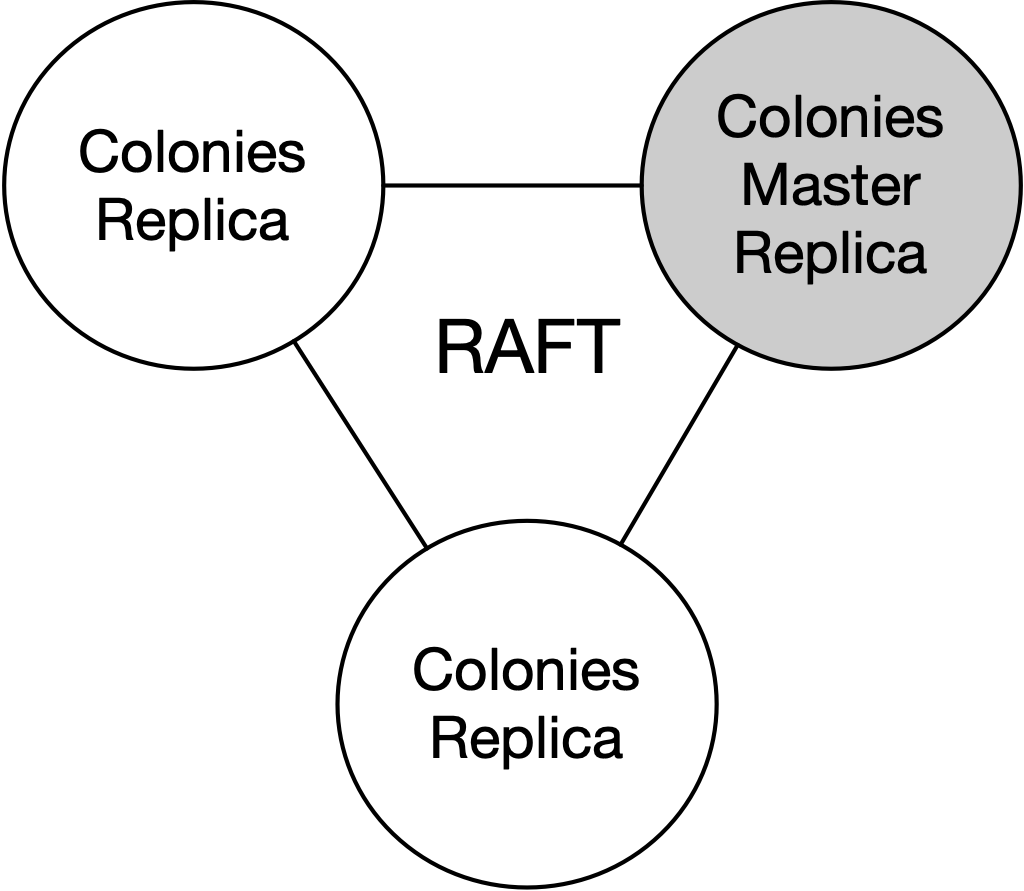
\includegraphics[scale=0.5]{raft.png}
	\caption{High-availability deployment of Colonies servcer.}
	\label{fig:ha_deployment}
\end{figure}

\subsubsection{Concurreny and synchronization}
Synchronization is esstential to prevent data inconsistency and race conditions when accessing shared resources concurrently with multiple threads. However, synchronization can also slows down execution as only one thread can access critical sections at a time. By carefully designing multithreaded applications and employing the right synchronization techniques, it possible to minimize the performance impact while still ensuring data consistency and correctness.  

The assign request allocates binds a process from the database to an executor. Given the multi-threaded nature of the Colonies server, it is essential that the assign request is synchronized to ensure that only one thread at a time can modify the database and update the process table, thus preventing multiple executors from being assigned to the same process. As only the assigned executor can modify a running process and only one executor must be assigned to a process, synchronization is required for the assign request. It is worth noting that synchronization is not necessary for other requests. For example, as the submit request only add new entries to the process table, there is no race conditions. The close request set the output of the function innovation and updates the process state to either successful or failed in the process table. Since there is only one assigned executor to a process there is no race conditions and consequently no need for synchronization.

To minimize downtime in the event of hardware or software failures, there is a need for high-availability and make use of a cluster of Colonies servers. If one Coloniser server crashes, an executor simply need to re-send a failed request, which will then be served by another Colonies server replica. However, by introducing multiple Colonies servers, there is again a risk of race conditions when assigning processes to executors. This means that the Colonies server replicas must coordintate which replica server incomming assign requests so that precisely one executor is assigned to a process.

Raft \cite{raft} is a consensus algorithm specifically designed to manage a replicated log within a distributed system. It functions within a cluster of servers, where a single server takes on the role of leader while the remaining servers act as followers. The leader is responsible for managing the replicated log, processing client requests, and replicating entries to the followers. Followers passively replicate the leader's log and participate in leader elections. The leadership can change over time due to elections triggered by timeouts or other factors.

Incorporting Raft with the Colonies framework allows incoming assign requests to be directed towards the leading Colonies server, thereby ensuring that only one Colonies server replica handles such requests. Figure \ref{fig:ha_deployment} shows an overview of a high-availability Colonies deployment. A new leader is elected in the event that a Colonies server replica fails. The Raft protocol also enables seamless updates to the Colonies server software by making it possible to upgrade each replica individually. As a result, Colonies becomes well-suited for Kubernetes deployments.

\subsubsection{Workflows}
A workflow is a series of tasks that need to be completed in a specific order. Workflows are often represented as directed acyclic graphs (DAGs), where nodes represent tasks and edges represent dependencies or data flow between tasks. 

\begin{figure}[h]
	\centering
    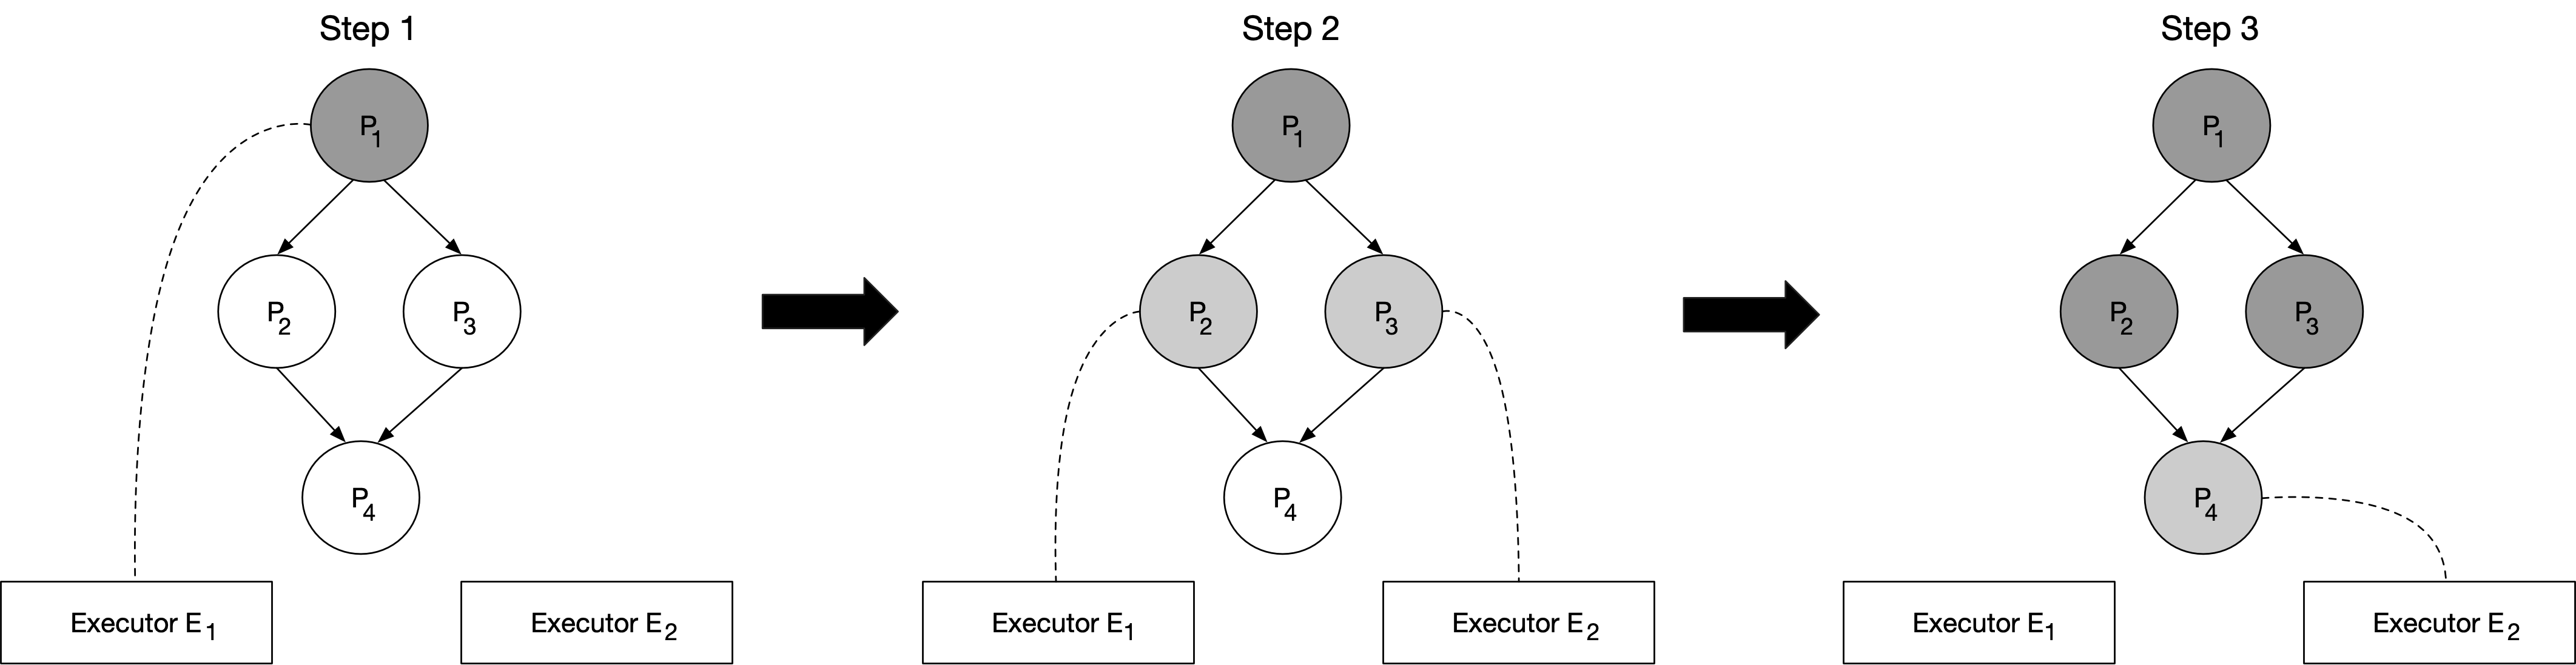
\includegraphics[scale=0.30]{workflow.png}
	\caption{cron management}
	\label{fig:fig3}
\end{figure}

\begin{table}[h]
	\caption{Function Specifications}
	\centering
	\begin{tabular}{llllll}
		\toprule
		\cmidrule(r){1-2}
        Function Spec & Function        & Executor Type & Priority & Max Exec Time & Max Retries \\
		\midrule
        $F_{1}$       & gen\_nums()     & Edge          & 1        & 200 s         & 5 \\
        $F_{2}$       & square()        & Cloud         & 1        & 200 s         & 5 \\
        $F_{3}$       & square()        & Cloud         & 1        & 200 s         & 5 \\
        $F_{4}$       & sum()           & Browser       & 1        & 200 s         & 5 \\
		\bottomrule
	\end{tabular}
	\label{tab:table}
\end{table}

\begin{table}[h]
	\caption{Snapshot of Process Table as in Step 2}
	\centering
	\begin{tabular}{llllll}
		\toprule
		\cmidrule(r){1-2}
        Process Id & Function Spec & Wait for Parents & Assigned Executor Id & State      & Priority Time \\
		\midrule
        $P_{1}$    & $F_{1}$       & $False$          & $E_{1}$              & Successful & 1679906715352024000 \\
        $P_{2}$    & $F_{2}$       & $False$          & $E_{1}$              & Running    & 1679906715353453000 \\
        $P_{3}$    & $F_{3}$       & $False$          & $E_{2}$              & Running    & 1679906715354286000 \\
        $P_{4}$    & $F_{4}$       & $True$           & -                    & Waiting    & 1679906715355188000 \\
		\bottomrule
	\end{tabular}
	\label{tab:table}
\end{table}

\begin{table}[h]
	\caption{Dependency Table}
	\centering
	\begin{tabular}{lll}
		\toprule
		\cmidrule(r){1-2}
        Process Id & Name       & Dependencies           \\
		\midrule
        $P_{1}$    & $Task_{1}$ & -                      \\
        $P_{2}$    & $Task_{2}$ & $Task_{1}$             \\
        $P_{3}$    & $Task_{3}$ & $Task_{1}$             \\
        $P_{4}$    & $Task_{4}$ & $Task_{2}$, $Task_{3}$ \\
		\bottomrule
	\end{tabular}
	\label{tab:table}
\end{table}
	
\begin{table}[h]
	\caption{Input/Output Table}
	\centering
	\begin{tabular}{lll}
		\toprule
		\cmidrule(r){1-2}
        Process Id & Input & Output \\
		\midrule
        $P_{1}$    & & [2,3] \\
        $P_{2}$    & 2 & 4 \\
        $P_{3}$    & 3 & 9 \\
        $P_{4}$    & [4,9] & 13 \\
		\bottomrule
	\end{tabular}
	\label{tab:table}
\end{table}

\subsubsection{Cron}
TODO
\begin{figure}[h]
	\centering
    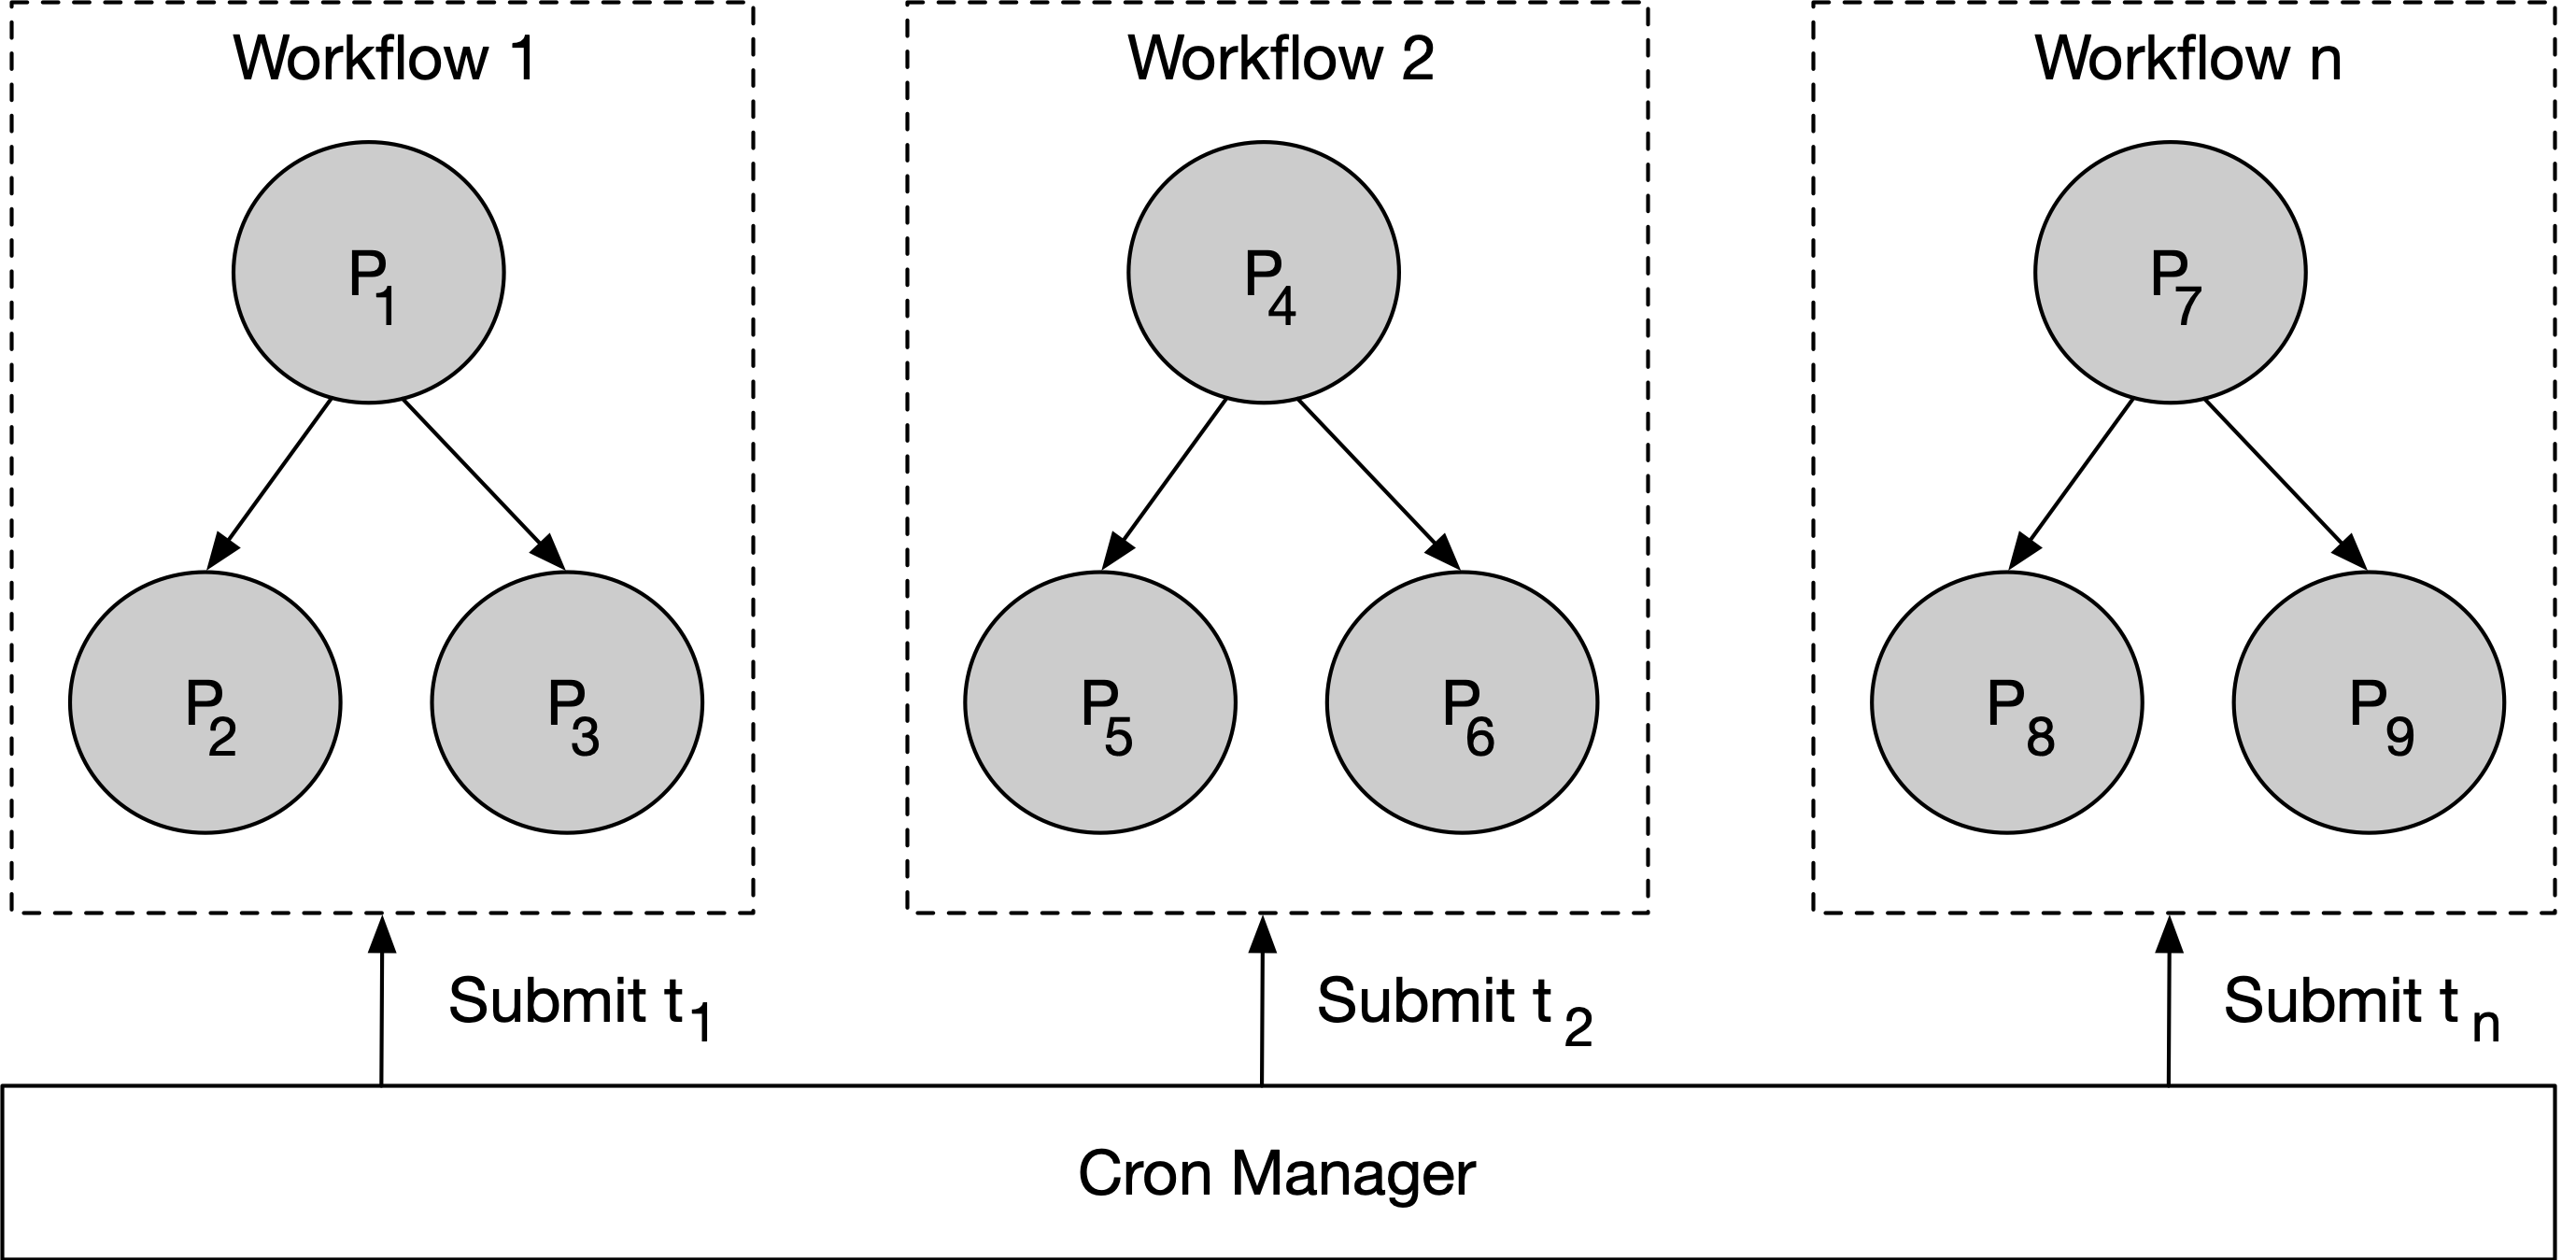
\includegraphics[scale=0.4]{cron.png}
	\caption{Sample figure caption.}
	\label{fig:fig1}
\end{figure}

\subsubsection{Generators}
TODO

\subsubsection{Zero-trust security}
TODO

\section{Evaluation}
\subsection{Implementation}

\bibliographystyle{unsrt}
\bibliography{references} 

\end{document}
